\documentclass{templateNote}
\usepackage{tcolorbox}
\usepackage{xcolor}
\usepackage{amssymb}
\usepackage{pgfplots}
\usepackage{tikz}

\newcommand{\destacar}[1]{ \colorbox{yellow}{#1}}

\begin{document}

\imagenlogo{img/logoUBB.png}
\universidad{Universidad del Bío-Bío pepito5}
\titulo{Apunte Economia} % Titulo
\asignatura{Economia 1} % Asignatura
\autor{
    \indent
    Marcelo \textsc{Paz}
}   
\portada
\margenes % Crear márgenes


\section{Conceptos básicos}
\begin{enumerate}
    \item \textbf{Economía:} Es la ciencia que estudia la forma en que los individuos y la sociedad efectúan las elecciones y decisiones para lograr el mejor uso posible de los recursos escasos, que tienen usos alternativos, para satisfacer sus necesidades ilimitadas.\\
    
    Enfoque de:
    \begin{enumerate}
        \item \textbf{Microeconómico:} estudia los comportamientos básicos de los
        agentes económicos individuales.
        \item \textbf{Macroeconómico:} analiza comportamientos agregados o
        globales, y se ocupa de temas como el empleo, la inflación o el
        producto total de una economía.
    \end{enumerate}
    
\end{enumerate}

\section{Microeconomía}
\indent
Es la disciplina que estudia la forma en la cual
se asignan los recursos escasos, entre los diversos usos que
compiten por ellos, con el proposito de satisfacer parte de los
deseos ilimitados de los individuos.\\
Actores:
\begin{enumerate}
    \item \textbf{Productores:} Recursos escasos, usos alternativos y múltiples.
    \item \textbf{Consumidores:} Necesidades múltiples, jerarquizables y progresivas. 
    \item \textbf{Relación de intercambio.}
\end{enumerate} 

\subsection{Aspectos}
\begin{enumerate}
    \item Los precios, cantidad, demanda de factores, determinantes del
    comportamiento.
    
    \item Fenómenos económicos desagregados de cada agente (empresa,
    consumidor, etc.) considerando las decisiones que toma cada uno
    para cumplir ciertos objetivos propios y considerando algunos
    supuestos de libre empresa o libre mercado.
\end{enumerate}
\subsection{Objetivos}
\begin{enumerate}
    \item Se considera a la microeconomía como el estudio de la asignación
de recursos escasos frente a necesidades múltiples.
    
    \item Uno de los principales objetivos de la microeconomía es analizar
los mecanismos que establecen los precios relativos de los bienes
y factores.
    
    \item La Microeconomía estudia el modo en que toman decisiones los
hogares y las empresas y la forma en que interactuan.
\end{enumerate}

\newpage
\section{Racionalidad económica}
\begin{enumerate}
    \item \textbf{Costo de oportunidad:} Es el \destacar{sacrificio asociado a una decisión.} Se
    busca maximizar o minimizar su función objetivo, sujeta a
    restricciones. Por lo general empleamos la matemática para
    representar estas situaciones.
    
    \item \textbf{Consumidor:} Su objetivo es \destacar{maximizar la utilidad} derivada del consumo de bienes, sujeta a precios y restricción presupuestaria. \\
\\
* Por tanto, el objetivo del consumidor se encuentra en consumir o alcanzar un nivel
de consumo determinado que nos permita llegar al nivel de utilidad
o bienestar deseado. \\

    \item \textbf{Productor:} Su objetivo es \destacar{maximizar los beneficios} (netos) de la producción (máximo ingreso, mínimo costo). \\
\end{enumerate}
* \textbf{Modelos económicos:} Es capaz de explicar y predecir los acontecimientos del mundo real (la mejor aproximación).

\section{Supuestos}
\begin{enumerate}
    \item \textbf{Ceteris paribus:} Las variables que no se están estudiando, se
    asumen constante (no varían) durante el periodo estudiado. En otras palabras, \colorbox{yellow}{las demás cosas se mantienen} 
    \colorbox{yellow}{constantes/iguales}.

    \item \textbf{Los agentes} toman decisiones para optimizar algo (maximizar o
    minimizar).

    \item \textbf{Distinción entre economía positiva (lo que es) y economía
    normativa (lo que debería ser).}

    \item \textbf{Mercado:} Lugar físico o virtual donde se encuentran los compradores y vendedores de un bien o servicio para realizar transacciones comerciales.\\ 
    \begin{enumerate}
        \item \textbf{El principio de la optimización:} Los individuos tratan de elegir las
        mejores pautas de consumo que estan a su alcance.

        \item \textbf{El principio de equilibrio:} Los precios se ajustan hasta que la
        cantidad que demanden los individuos de una cosa es igual a la
        que se ofrece.

        \item \textbf{El consumidor elige la cesta de consumo} que prefiere dado el
        conjunto de combinaciones de bienes, y la optimización que
        puede alcanzar.

        \item \textbf{Los consumidores tienen preferencias} sobre algunos bienes y servicios.
        
    \end{enumerate}
* Lo anterior se refiere a que los consumidores, dados los precios
de estos bienes preferirán una canasta sobre la otra.
\end{enumerate}

\section{Montaña de la felicidad}
\indent

La montaña de la felicidad es una representación gráfica de las preferencias de un individuo.\\
\begin{itemize}
    \item Donde $U_5$ es la mayor utilidad y $U_1$ la menor utilidad.
    \item Cada nivel esta limitado por la restricción presupuestaria.
\end{itemize}

\begin{equation*}
    U_5 > U_4 > U_3 > U_2 > U_1
\end{equation*}

\begin{figure}[H]
    \centering
    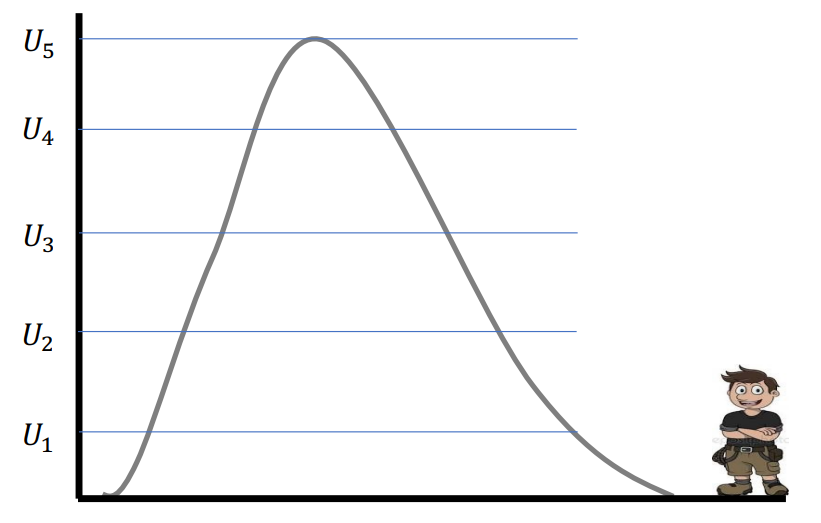
\includegraphics[scale=0.5]{img/Mountain.png}
    \caption{Montaña de la felicidad}
\end{figure}

\section{Mercado}

\begin{enumerate}
    \item \textbf{Monopolio(único vendedor):}Es una estructura de mercado
    caracterizada por la presencia de una \destacar{única empresa}, que
    produce un bien homogéneo y que \destacar{define sus precios}, calidad,
    cantidad y mercado.

    \item \textbf{Competencia perfecta:}
    \begin{itemize}
        \item Aquella en que hay varios productores que \destacar{compiten en igualdad
        de condiciones} para atraer la demanda de los consumidores.

        \item Una economía liberal es el sistema ideal de desarrollo para los
        mercados y lograr satisfacer al consumidor
    \end{itemize}

\newpage
    \item \textbf{Oligopolio:}
    \begin{itemize}
        \item Del griego, pocos vendedores. \destacar{Se supone que hay pocas
        empresas, pero de tal} \destacar{forma que, ninguna de ellas puede
        controlar totalmente el mercado.}

        \item Hay por ello una constante lucha entre las mismas, para poder
        llevarse la mayor parte de la cuota de mercado.

        \item Así las empresas toman decisiones estratégicas, teniendo
        encuenta las fortalezas y debilidades de la estructura empresarial
        de cada una.        
    \end{itemize}

    \item \textbf{Competencia monopolística:}
    \begin{itemize}
        \item Es una estructura de mercado caracterizada por la presencia de
        muchas empresas que venden productos homogéneos,
        sustitutivos cercanos, pero distintos, entre sí.

        \item Al tratarse de productos heterogéneos, cada productor tiene un
        cierto poder de mercado sobre el bien que produce, por lo que la
        competencia monopolística puede definirse como una estructura
        de mercado intermedia entre monopolio en competencia
        perfecta.
    \end{itemize}
\end{enumerate}

\section{Grandes Interrogantes}
\subsection{¿Qué y cuánto producir?}
\indent
Elección de bienes y servicios a ofertar según las necesidades.

\subsection{¿Cómo producir?}
\indent
Elección de la forma a utilizar para transformar los bienes.

\subsection{¿Para quién producir?}
\indent
Decidir sobre la distribución de la producción entre los individuos.

\newpage
\section{Ejercicios}
\subsection{Problema de maximización visto en clase}
\begin{itemize}
    \item Sea la función de utilidad $U(q_1,q_2) = q_1 \cdot q_2$
    \item La renta $Y = 200$.
    \item Los precios $p_1 = 4$ y $p_2 = 1$.
\end{itemize}

Entonces:
\begin{equation*}
    \begin{split}
        max_{q_1, q_2} (q_1 \cdot q_2) \\
        \text{s.a.} \quad 4q_1 + q_2 = 200 \\
    \end{split}
\end{equation*}
* s.a. = sujeto a.\\
\begin{itemize}
    \item \textbf{Paso 1:} Resolver la restricción de presupuesto para $q_2$.
    \begin{align*}
        q_2 &= 200 -4q_1
    \end{align*}
    
    \item \textbf{Paso 2:} Reemplazar la restricción en la función de utilidad.
    \begin{align*}
        max_{q_1} (q_1) &= q_1 \cdot (200 -4q_1) \\
        &= 200q_1 -4 {q_1}^2
    \end{align*}
    
    \item \textbf{Paso 3:} Calcular las condiciones de primer orden con respecto a $q_1$.
    \begin{align*}
        \frac{\mathrm{d} U(q_1)}{\mathrm{d}q_1} &= 200 -8q_1 = 0 \Leftrightarrow {q_1}^* = 25
    \end{align*}
    
    \item \textbf{Paso 4:} Utilizar las condiciones de primer orden para despejar $q_2$.
    \begin{align*}
        {q_2}^* &= 200 -4 \times 25 \\
        &= 100 \\
    \end{align*}
    $\therefore \quad$ la utilidad del problema de maximización es:
    \begin{align*}
        U({q_1}^*, {q_2}^*) &= 25 \times 100 \\
        &= 2500
    \end{align*}
    
\end{itemize}

\newpage
\subsection{Material Ayudantia 4}
\subsubsection{Ejercicio 1}
\indent
Explique el paso a paso del Método de Sustitución. Además exprese la ecuación de
optimización y la restricción presupuestaria
\begin{itemize}
    \item \textbf{Paso 1:} Despejar una de las variables de la restricción presupuestaria.
    \item \textbf{Paso 2:} Reemplazar la variable despejada en la función de utilidad.
    \item \textbf{Paso 3:} Calcular la condición de primer orden con respecto a la variable que no se despejo.
    \item \textbf{Paso 4:} Despejar la variable que no se despejo en el paso 1.
    \item \textbf{Paso 5:} Reemplazar el resultado del paso 4 en la restricción presupuestaria para obtener la utilidad máxima.
\end{itemize}

\subsubsection{Ejercicio 2}
\begin{itemize}
    \item Sea la función de utilidad $U(q_1,q_2) = q_1 \cdot q_2$
    \item La renta $Y = 1200$.
    \item Los precios $p_1 = 6$ y $p_2 = 4$.
\end{itemize}

Entonces:
\begin{equation*}
    \begin{split}
        max_{q_1, q_2} (q_1 \cdot q_2) \\
        \text{s.a.} \quad 6q_1 + 4q_2 = 1200
    \end{split}
\end{equation*}
\begin{align*}
    q_2 &= 300 - \frac{3}{2}q_1 \\
    \\
    max_{q_1} (q_1) &= q_1 \cdot (300 - \frac{3}{2}q_1) \\
    &= 300q_1 - \frac{3}{2} {q_1}^2 \\
    \\
    \frac{\mathrm{d} U(q_1)}{\mathrm{d}q_1} &= 300 - 3q_1 = 0 \Leftrightarrow {q_1}^* = 100 \\
    \\
    {q_2}^* &= 300 - \frac{3}{2} \times 100 \\
    &= 150 \\
    \\
    \therefore \quad U({q_1}^*, {q_2}^*) &= 100 \times 150 \\
    &= 15000
\end{align*}

\newpage
\subsubsection{Ejercicio 3}
Suponga que un consumidor cuenta con una renta de 600 unidades monetarias, que puede
gastar únicamente entre dos bienes $A$ y $B$. El precio del bien $A$ es $P_a = 2$, y del bien $B$ es
$P_b = 3$

\textbf{a)} Indique cuál será la función de su restricción presupuestaria.
\begin{align*}
    2A + 3B &= 600
\end{align*}

\textbf{b)} ¿Qué número de unidades del bien $A$ podrá adquirir si dedica toda su renta a
comprar dicho bien?
Sea $B = 0$.
\begin{align*}
    2A + 3(0) &= 2A = 600 \Leftrightarrow A = 300
\end{align*}

\textbf{c)} ¿Cuánto podrá comprar del bien $B$ si no compra nada del bien $A$?
Sea $A = 0$.
\begin{align*}
    2(0) + 3B &= 3B = 600 \Leftrightarrow B = 200
\end{align*}

\textbf{d)} Represente gráficamente la restricción presupuestaria.
\begin{figure}[H]
    \centering
    \begin{tikzpicture}
        \begin{axis}[
            axis lines = left,
            xlabel style={at={(rel axis cs:1.04,0)}, anchor=west},
            ylabel style={rotate =-90 ,at={(rel axis cs:0.10,1.03)}, anchor=south},
            xmax = 500,
            ymax = 350,
            height = 10cm,
            width = 10cm,
            xmin = 0,
            ymin = 0,
            xlabel = $A$,
            ylabel = $B$,
        ]
        \addplot [
            domain=0:300, 
            samples=100, 
            color=red,
        ]
        {200-2/3*x};
        \addlegendentry{$200-\frac{2}{3}A$}
        \end{axis}
    \end{tikzpicture}
    \caption{Restricción presupuestaria}
\end{figure}

\newpage
\textbf{e)}  Si la renta del individuo aumenta hasta hasta $R = 900$, ¿Qué pasaría con la
restricción presupuestaria? Representar gráficamente.

Sea $R = 900$.
\begin{align*}
    2A + 3B &= 900 \\
    3B &= 900 - 2A \\
    B &= 300 - \frac{2}{3}A
\end{align*}

Sea $A = 0$.
\begin{align*}
    B &= 300 - \frac{2}{3} \times 0 \\
    &= 300
\end{align*}

Sea $B = 0$.
\begin{align*}
    2A &= 900 \\
    A &= 450
\end{align*}

\begin{figure}[H]
    \centering
    \begin{tikzpicture}
        \begin{axis}[
            axis lines = left,
            xlabel style={at={(rel axis cs:1.04,0)}, anchor=west},
            ylabel style={rotate =-90 ,at={(rel axis cs:0.10,1.03)}, anchor=south},
            xmax = 500,
            ymax = 350,
            height = 10cm,
            width = 10cm,
            xmin = 0,
            ymin = 0,
            xlabel = $A$,
            ylabel = $B$,
        ]
        \addplot [
            domain=0:300, 
            samples=100, 
            color=red,
        ]
        {200-2/3*x};

        \addplot [
            domain=0:450, 
            samples=100, 
            color=blue,
        ]
        {300-2/3*x};
        \draw[->, thick] (axis cs:160,120) -- (axis cs:230,120);
        \draw (axis cs:175,125) node[above] {$R = 900$};
        \addlegendentry{$200-\frac{2}{3}A$}
        \addlegendentry{$300-\frac{2}{3}A$}
        \end{axis}
    \end{tikzpicture}
    \caption{Restricción presupuestaria}
\end{figure}

\newpage
\textbf{f)} Suponga ahora que, en lugar del incremento de la renta, el precio del bien $A$ se
duplica. Represente la nueva restricción presupuestaria.

Sea $P_a = 4$.
\begin{align*}
    4A + 3B &= 600 \\
    3B &= 600 - 4A \\
    B &= 200 - \frac{4}{3}A
\end{align*}

Sea $A = 0$.
\begin{align*}
    B &= 200 - \frac{4}{3} \times 0 \\
    &= 200
\end{align*}

Sea $B = 0$.
\begin{align*}
    4A &= 600 \\
    A &= 150
\end{align*}

\begin{figure}[H]
    \centering
    \begin{tikzpicture}
        \begin{axis}[
            axis lines = left,
            xlabel style={at={(rel axis cs:1.04,0)}, anchor=west},
            ylabel style={rotate =-90 ,at={(rel axis cs:0.10,1.03)}, anchor=south},
            xmax = 350,
            ymax = 250,
            height = 10cm,
            width = 10cm,
            xmin = 0,
            ymin = 0,
            xlabel = $A$,
            ylabel = $B$,
        ]
        \addplot [
            domain=0:300, 
            samples=100, 
            color=red,
        ]
        {200-2/3*x};

        \addplot [
            domain=0:150, 
            samples=100,
            color=blue,
        ]
        {200-4/3*x};
        \draw[<-, thick] (axis cs:110,75) -- (axis cs:160,75);
        \draw (axis cs:120,80) node[above] {$P_a = 4$};
        \addlegendentry{$200-\frac{2}{3}A$}
        \addlegendentry{$200-\frac{4}{3}A$}
        \end{axis}
    \end{tikzpicture}
    \caption{Restricción presupuestaria}
\end{figure}

\newpage
\subsubsection{Ejercicio 4}
\begin{itemize}
    \item Sea la función de utilidad $U(X,Y) = 10 X \cdot Y$
    \item $m = xp_x + yp_y$
    \item Los precios $p_x = 4$ y $p_y = 3$.
    \item La renta $m = 300$.
\end{itemize}

Entonces:
\begin{equation*}
    \begin{split}
        max_{X, Y} (10 X \cdot Y) \\
        \text{s.a.} \quad 4X + 3Y = 300
    \end{split}
\end{equation*}

\begin{align*}
    Y &= 100 - \frac{4}{3}X \\
    \\
    max_{X} (10 X \cdot (100 - \frac{4}{3}X)) &= 1000X - \frac{40}{3} {X}^2 \\
    \\
    \frac{\mathrm{d} U(X)}{\mathrm{d}X} &= 1000 - \frac{80}{3}X = 0 \Leftrightarrow {X}^* = 37.5 \\
    \\
    {Y}^* &= 100 - \frac{4}{3} \times 37.5 \\
    &= 50 \\
    \\
    \therefore \quad U({X}^*, {Y}^*) &= 37.5 \times 50 \\
    &= 1875
\end{align*}

\subsubsection{Ejercicio 5}
\indent
¿En qué caso se maximiza la utilidad del consumidor?

\textbf{R:} Cuando la utilidad marginal es igual al precio.

Cuando la tasa a la que se está dispuesto a cambiar $q_1$ por $q_2$ es igual a la tasa a la que
puedes cambiarlos.

\begin{equation*}
    TMS = TMT \Leftrightarrow - \frac{U_1}{U_2} = - \frac{p_1}{p_2} \Leftrightarrow \frac{U_1}{U_2} = \frac{p_1}{p_2}
\end{equation*}
* \textbf{TMS} = Tasa marginal de sustitución.\\
* \textbf{TMT} = Tasa marginal de transformación.\\
* $\mathbf{U_1}$ = Utilidad marginal de $q_1$.\\
* $\mathbf{U_2}$ = Utilidad marginal de $q_2$.\\
* $\mathbf{p_1}$ = Precio de $q_1$.\\
* $\mathbf{p_2}$ = Precio de $q_2$.\\

% \newpage
\end{document}
